\section{Data Collection and Representation}
\subsection{Data Sources \& Collection}

\begin{frame}{Data Sources}
    \begin{itemize}
        \item Web APIs and web scraping
        \item Batch ingestion vs.\ real-time streaming pipelines
        \item Public ML repositories (Kaggle, UCI Machine Learning Repository)
        \item Administrative and survey microdata (e.g.\ DHS/MICS-style datasets), typically collected under a complex survey design with sampling weights
    \end{itemize}
\end{frame}


\begin{frame}{Data Types}
    \begin{itemize}
        \item Tabular data
        \item Unstructured data: text, images, audio
        \item Time-series data
        \item Graph / network data
        \item Structured vs.\ semi-structured: relational tables vs.\ JSON-style API responses
    \end{itemize}
\end{frame}


\subsection{Linear Algebra Foundations \& Mathematical Representation}


\begin{frame}{Feature Vectors}
    \begin{sitemize}
        \item Each data point is represented as a $d$-dimensional feature vector.
        \item For the $i$-th instance in the dataset,
        $$x^{(i)} = \begin{bmatrix} x^{(i)}_1 & x^{(i)}_2 & \dots & x^{(i)}_d \end{bmatrix}^T \in \mathbb{R}^d$$
        \item The superscript $(i)$ indexes the instance; the subscript indexes the feature.
    \end{sitemize}
\end{frame}


\begin{frame}{The Design Matrix}
    \begin{sitemize}
        \item Stacking $n$ instances gives an $n \times d$ design matrix,
        $$X = \begin{bmatrix} x^{(1)T} \\ x^{(2)T} \\ \vdots \\ x^{(n)T} \end{bmatrix} = \begin{bmatrix} x_{11} & x_{12} & \dots & x_{1d} \\ x_{21} & x_{22} & \dots & x_{2d} \\ \vdots & \vdots & \ddots & \vdots \\ x_{n1} & x_{n2} & \dots & x_{nd} \end{bmatrix} \in \mathbb{R}^{n \times d}$$
        \item Row $i$ of $X$ is the transpose of instance $i$'s feature vector, $x^{(i)T}$; column $j$ holds every instance's value for feature $j$.
    \end{sitemize}
\end{frame}


\begin{frame}{Target Vector}
    \begin{sitemize}
        \item Target variables are collected into a vector $y \in \mathbb{R}^n$, one entry per instance.
        \item Continuous values for regression (e.g.\ price, temperature); discrete class labels for classification (e.g.\ spam / not spam).
    \end{sitemize}
\end{frame}


\begin{frame}{Practical Scenario: Real Estate Price Prediction}
    \begin{sitemize}
        \item Each row of $X$ is one house: $x^{(i)} = [x_{\text{sqft}}, x_{\text{beds}}, x_{\text{baths}}, x_{\text{zip}}]^T$.
        \item For three houses,
        $$X = \begin{bmatrix} 1400 & 3 & 2 & 10001 \\ 2200 & 4 & 3 & 10002 \\ 950 & 2 & 1 & 10001 \end{bmatrix}, \qquad y = \begin{bmatrix} 310 \\ 480 \\ 205 \end{bmatrix} \text{(\$1000s)}$$
        \item The model learns a mapping from each row of $X$ to the corresponding entry of $y$.
    \end{sitemize}
\end{frame}


\section{Features and Feature Engineering Basics}

\subsection{Feature Taxonomy}


\begin{frame}{Feature Taxonomy}
    \begin{itemize}
        \item \textbf{Categorical:} Nominal (unordered, e.g.\ color, region), Ordinal (ordered, e.g.\ education level)
        \item \textbf{Numerical:} Discrete (integer counts), Continuous (real numbers)
        \item \textbf{Binary:} Logical indicators, $0$ or $1$
    \end{itemize}
\end{frame}


\subsection{Categorical Encoding Techniques}


\begin{frame}{One-Hot Encoding (Dummy Variables)}
    \begin{sitemize}
        \item Expands a categorical column with $k$ levels into $k$ (or $k-1$) binary indicator columns.
        \item Used for nominal data with distance- or gradient-based algorithms (Linear Regression, Neural Networks, SVMs), to avoid implying an ordinal relationship that doesn't exist.
        \item Example: \texttt{Color} $\in \{$Red, Blue, Green$\}$ becomes \texttt{Is\_Red}, \texttt{Is\_Blue}, \texttt{Is\_Green}.
    \end{sitemize}
\end{frame}


\begin{frame}{Ordinal / Label Encoding}
    \begin{sitemize}
        \item Maps ordered categories to an integer sequence, $0, 1, 2, \dots$
        \item Appropriate for genuinely ordinal features, or for tree-based algorithms (Random Forests, XGBoost) that split on integers efficiently without expanding dimensionality.
        \item Example: satisfaction responses [Poor, Satisfactory, Excellent] $\to$ [0, 1, 2].
    \end{sitemize}
\end{frame}


% \begin{frame}{Target / Mean Encoding}
    % \begin{sitemize}
    %     \item Replaces each category level with the mean of the target variable for that category.
    %     \item A cheaper alternative for the same problem is frequency encoding: replacing each level with its count or relative frequency.
    %     \item Useful for high-cardinality nominal variables, where one-hot encoding would create a sparse, high-dimensional matrix.
    %     \item Example: encoding $10{,}000$ unique \texttt{Zip\_Code} values by the average house price in that zip code.
    % \end{sitemize}
    % \begin{block}{Watch for Leakage}
    % Target statistics must be computed out-of-fold — using only training-fold data. Computing them on the full dataset before splitting leaks target information into the features. The same principle resurfaces with scaling and imputation.
    % \end{block}
% \end{frame}


\subsection{Feature Scaling \& Normalization}


\begin{frame}{Standardization ($Z$-Score Scaling)}
    \begin{sitemize}
        \item Formula: $x' = \dfrac{x - \mu}{\sigma}$, giving $\mu = 0$, $\sigma = 1$.
        \item Needed for algorithms sensitive to scale and to gradient descent step size (KNN, Linear/Logistic Regression, SVMs, Neural Networks).
        \item Example: bringing \texttt{Age} ($0$--$100$ years) and \texttt{Annual Income} (\$10,000--\$1,000,000) onto a common scale.
        \item Fit $\mu$ and $\sigma$ on the training set only, then apply to validation/test — the same leakage principle as target encoding.
    \end{sitemize}
\end{frame}


\begin{frame}{Min-Max Scaling}
    \begin{sitemize}
        \item Formula: $x' = \dfrac{x - x_{\min}}{x_{\max} - x_{\min}}$, bounding data to $[0,1]$.
        \item Used for non-Gaussian features needing a bounded range, or to preserve zero values in sparse matrices.
        \item Example: normalizing image pixel intensities ($0$--$255$) before neural network training.
        \item Terminology note: this and standardization are column-wise \emph{scaling}. Row-wise \emph{normalization} (e.g.\ rescaling each instance vector to unit $L_2$ norm) is a distinct operation — the two terms get conflated often.
    \end{sitemize}
\end{frame}


\begin{frame}{Robust Scaling (Median \& IQR)}
    \begin{sitemize}
        \item Formula: $x' = \dfrac{x - \text{Median}}{\text{IQR}}$.
        \item Used when scale-sensitive algorithms meet data with legitimate extreme values that would distort mean/variance-based scaling.
        \item Example: scaling executive compensation data with a heavy upper tail.
    \end{sitemize}
\end{frame}


\section{Data Preprocessing and Cleaning}

\subsection{Handling Missing Values}


\begin{frame}{Missingness Mechanisms}
    \begin{sitemize}
        \item \textbf{MCAR} (Missing Completely at Random): missingness is independent of both observed and unobserved data.
        \item \textbf{MAR} (Missing at Random): missingness depends on observed data, but not on the missing value itself.
        \item \textbf{MNAR} (Missing Not at Random): missingness depends on the unobserved value itself (e.g.\ high earners skipping the salary question).
    \end{sitemize}
\end{frame}


\begin{frame}{Deletion Strategies}
    \begin{sitemize}
        \item \textbf{Listwise deletion:} drop entire rows with any missing entry. Reasonable under MCAR with minimal missingness ($<2$--$5\%$); risky under MAR/MNAR, where it introduces bias and shrinks the sample.
        \item \textbf{Pairwise deletion:} use all available data for each calculation (e.g.\ each pairwise correlation) rather than discarding a row entirely. Avoids losing data but can leave summary statistics computed on inconsistent subsamples.
    \end{sitemize}
\end{frame}


\begin{frame}{Simple Imputation}
    \begin{sitemize}
        \item \textbf{Mean / Median / Mode Imputation:} replace missing entries with a global summary statistic — median for numerical/skewed features, mode for categorical.
        \item Appropriate for baseline modeling with minimal MCAR missingness ($<5\%$).
    \end{sitemize}
\end{frame}


\begin{frame}{Model-Based Imputation}
    \begin{sitemize}
        \item \textbf{$k$-Nearest Neighbors (KNN) Imputation:} imputes using feature distance to neighboring rows. Suited to tabular data with moderate missingness ($5$--$15\%$) where features are correlated.
        \item \textbf{MICE} (Multivariate Imputation by Chained Equations): models each variable with missing values as a function of the others, iteratively. Suited to high-stakes statistical/clinical modeling under MAR, with missingness spread across multiple features.
        \item Fit both on the training fold only, then apply to validation/test — the same leakage principle as target encoding.
    \end{sitemize}
\end{frame}


\subsection{Handling Outliers}


\begin{frame}{Outlier Detection: IQR and $Z$-Score}
    \begin{sitemize}
        \item \textbf{Tukey's IQR rule:} flag points outside $[Q1 - 1.5 \times \text{IQR}, \, Q3 + 1.5 \times \text{IQR}]$.
        \item \textbf{$Z$-score rule:} flag points where $|z| = \left|\dfrac{x - \mu}{\sigma}\right| > 3$ (or another chosen threshold).
        \item $Z$-score reuses the standardization formula from Section 2; it assumes roughly normal data and is sensitive to the same outliers it's trying to detect, since they inflate $\mu$ and $\sigma$ — the IQR rule is more robust to that feedback loop.
    \end{sitemize}
\end{frame}


\begin{frame}{Outlier Detection: Isolation Forest}
    \begin{sitemize}
        \item Model-based detection: measures how quickly an instance is isolated by random tree partitions — outliers isolate in fewer splits.
        \item Suited to high-dimensional tabular data, where single-feature rules (IQR, $Z$-score) miss multivariate anomalies.
        \item Example: credit card fraud detection, where a fraudulent transaction may look normal on any one feature but anomalous jointly.
    \end{sitemize}
\end{frame}


\begin{frame}{Outlier Treatment}
    \begin{sitemize}
        \item \textbf{Trimming / culling:} remove verified, corrupt outlier rows.
        \item \textbf{Winsorization (capping):} replace extreme values with a boundary percentile (e.g.\ 1st/99th), preserving sample size while limiting the influence of tail values on parametric regression coefficients.
    \end{sitemize}
\end{frame}


\subsection{Data Integrity \& Hygiene}


\begin{frame}{Data Integrity \& Hygiene}
    \begin{itemize}
        \item Deduplication of redundant rows
        \item Structural corrections: unit conversions, standardizing date-time strings, fixing casing errors
    \end{itemize}
\end{frame}


\section{Exploratory Data Analysis (EDA) \& Data Visualization}

\subsection{Summary Statistics \& Central Tendency}


\begin{frame}{Summary Statistics}
    \begin{itemize}
        \item \textbf{Central tendency:} Mean, Median, Mode
        \item \textbf{Dispersion:} Variance, Standard Deviation, Interquartile Range (IQR)
        \item First step of EDA: establishes central values, spread, and baseline data health before any modeling
    \end{itemize}
\end{frame}


\begin{frame}{Distribution Shape}
    \begin{sitemize}
        \item Compare mean and median to detect skew: right-skewed income data shows Mean (\$85{,}000) well above Median (\$52{,}000).
        \item A long right tail (a few very high earners) pulls the mean up without moving the bulk of the distribution — visible directly in a histogram.
    \end{sitemize}
    \begin{figure}
    \centering
% --- ggplot2 (R) equivalent, for reference ---
% income_df <- data.frame(income = c(rep(10,15), rep(30,25), rep(50,20),
%                                     rep(70,12), rep(90,8), rep(110,5),
%                                     rep(130,3), rep(150,2)))
% ggplot(income_df, aes(x = income)) +
%   geom_histogram(binwidth = 20, fill = "steelblue", color = "white") +
%   labs(x = "Income ($1000s)", y = "Frequency")
        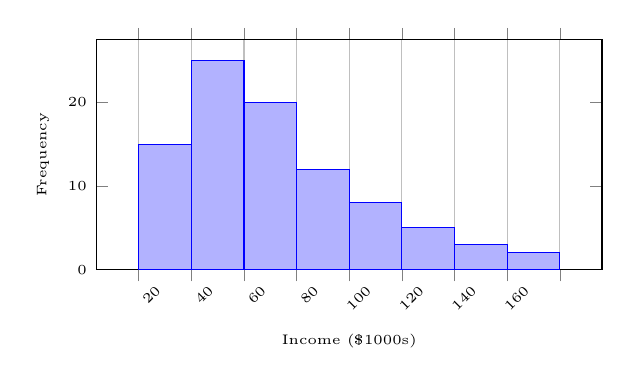
\begin{tikzpicture}
                \begin{axis}[
                    width=8cm, height=4.5cm,
                    font=\tiny,
                    xlabel={Income (\$1000s)},
                    ylabel={Frequency},
                    ybar interval,
                    xtick=data,
                    x tick label style={rotate=45,anchor=east},
                    tick label style={font=\tiny},
                    ymin=0,
                ]
                    \addplot table[row sep=\\] {
                        x y \\
                        20 15 \\
                        40 25 \\
                        60 20 \\
                        80 12 \\
                        100 8 \\
                        120 5 \\
                        140 3 \\
                        160 2 \\
                        180 0 \\
                    };
                \end{axis}
        \end{tikzpicture}
    \end{figure}
\end{frame}


\subsection{Groupwise Analysis \& Segment Distributions}

\begin{frame}{Groupwise Boxplots}
    \begin{sitemize}
        \item Compare a continuous feature's distribution across discrete groups: median, spread, and outliers per group, side by side.
        \item Example: salary distributions by job level, or recovery times by treatment arm (Placebo, Drug A, Drug B).
        \item Reveals sub-group variance and median shifts that a single overall summary statistic would hide.
    \end{sitemize}
    \begin{figure}
    \centering
% --- ggplot2 (R) equivalent, for reference ---
% salary_df <- data.frame(level = rep(c("Entry","Mid","Senior"), each = 50),
%                          salary = c(rnorm(50, 45, 8), rnorm(50, 66, 10),
%                                     rnorm(50, 97, 15)))
% ggplot(salary_df, aes(x = level, y = salary, color = level)) +
%   geom_boxplot() +
%   labs(x = NULL, y = "Salary ($1000s)") +
%   theme(legend.position = "none")
        \begin{tikzpicture}
            \begin{axis}[
                width=4.5cm, height=4cm,
                font=\tiny,
                ylabel={Salary (\$1000s)},
                boxplot/draw direction=y,
                xtick={1,2,3},
                xticklabels={Entry,Mid,Senior},
                tick label style={font=\tiny},
            ]
                \addplot+[boxplot prepared={
                    median=45, upper quartile=52, lower quartile=38,
                    upper whisker=65, lower whisker=30}] coordinates {};
                \addplot+[boxplot prepared={
                    median=65, upper quartile=75, lower quartile=58,
                    upper whisker=90, lower whisker=48}] coordinates {};
                \addplot+[boxplot prepared={
                    median=95, upper quartile=110, lower quartile=85,
                    upper whisker=130, lower whisker=70}] coordinates {};
            \end{axis}
        \end{tikzpicture}
    \end{figure}
\end{frame}


\begin{frame}{Groupwise Aggregations \& Contingency Tables}
    \begin{sitemize}
        \item Cross-tabulate a categorical outcome against a categorical predictor to segment behavior by group.
        \item Example: churn status against subscription tier (Basic, Pro, Enterprise), to find segment-specific churn rates.
        \item Watch for Simpson's Paradox: an association that holds within every subgroup can reverse when the subgroups are pooled.
    \end{sitemize}
\end{frame}


\subsection{Bivariate \& Multivariate Structural Analysis}


\begin{frame}{Scatter Plots \& Trendlines}
    \begin{sitemize}
        \item Examine pairwise relationships between a continuous feature and the target.
        \item Example: \texttt{House\_Size} vs.\ \texttt{Sales\_Price}, with a fitted trendline to check linearity.
    \end{sitemize}
    \begin{figure}
        \centering
        % --- ggplot2 (R) equivalent, for reference ---
        % house_df <- data.frame(size = seq(800, 2600, by = 200),
        %                         price = c(150,180,210,230,270,300,330,350,400,420))
        % ggplot(house_df, aes(x = size, y = price)) +
        %   geom_point() +
        %   geom_smooth(method = "lm", se = FALSE) +
        %   labs(x = "House Size (sqft)", y = "Price ($1000s)")
        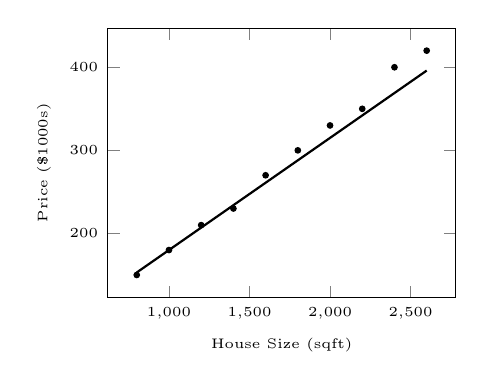
\begin{tikzpicture}
            \begin{axis}[
                width=6cm, height=5cm,
                font=\tiny,
                xlabel={House Size (sqft)},
                ylabel={Price (\$1000s)},
                tick label style={font=\tiny},
            ]
                \addplot[only marks, mark size=1pt] coordinates {
                (800,150) (1000,180) (1200,210) (1400,230)
                (1600,270) (1800,300) (2000,330) (2200,350)
                (2400,400) (2600,420)
                };
                \addplot[domain=800:2600, samples=2, thick] {0.135*x + 45};
            \end{axis}
        \end{tikzpicture}
    \end{figure}
\end{frame}


\begin{frame}{Correlation Matrices \& Heatmaps}
    \begin{sitemize}
        \item Metrics: Pearson linear correlation ($r$), Spearman rank correlation.
        \item Screen features for multicollinearity before training a model.
        \item Example: pairwise correlations among \texttt{Height}, \texttt{Weight}, \texttt{BMI}, \texttt{Waist\_Circumference} to flag collinear pairs ($r > 0.85$).
    \end{sitemize}
    \begin{figure}
        \centering
% --- ggplot2 (R) equivalent, for reference ---
% library(reshape2)
% corr_mat <- cor(body_df[, c("Height","Weight","BMI","Waist")])
% ggplot(melt(corr_mat), aes(Var1, Var2, fill = value)) +
%   geom_tile() +
%   scale_fill_viridis_c(limits = c(-1, 1)) +
%   labs(x = NULL, y = NULL, fill = "r")
        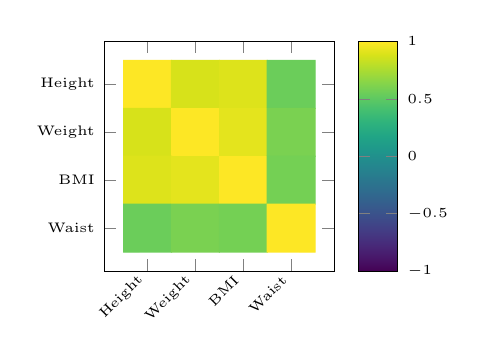
\begin{tikzpicture}
            \begin{axis}[
                width=4.5cm, height=4.5cm,
                font=\tiny,
                colormap/viridis,
                colorbar,
                colorbar style={font=\tiny},
                xtick=data, ytick=data,
                xticklabels={Height,Weight,BMI,Waist},
                yticklabels={Height,Weight,BMI,Waist},
                x tick label style={rotate=45,anchor=east},
                tick label style={font=\tiny},
                point meta min=-1, point meta max=1,
            ]
                \addplot[matrix plot, mesh/cols=4, point meta=explicit] table[meta=C, row sep=\\] {
                x y C \\
                0 0 1.00 \\
                1 0 0.88 \\
                2 0 0.90 \\
                3 0 0.55 \\
                0 1 0.88 \\
                1 1 1.00 \\
                2 1 0.92 \\
                3 1 0.60 \\
                0 2 0.90 \\
                1 2 0.92 \\
                2 2 1.00 \\
                3 2 0.58 \\
                0 3 0.55 \\
                1 3 0.60 \\
                2 3 0.58 \\
                3 3 1.00 \\
                };
            \end{axis}
        \end{tikzpicture}
    \end{figure}
\end{frame}



% \begin{frame}{High-Dimensional Visual Inspection}
% \begin{sitemize}
%     \item High-level overview of visualizing high-dimensional data in 2D (PCA, $t$-SNE, UMAP formulations covered in the dedicated dimensionality reduction lecture).
%     \item Used for a quick visual check of class separability or cluster structure before building a classifier.
% \end{sitemize}
% \begin{figure}
% \centering
% --- ggplot2 (R) equivalent, for reference ---
% proj_df <- data.frame(pc1 = c(1,1.5,0.8,1.2,1.6,0.9, 4,4.3,3.8,4.5,4.1,3.9),
%                        pc2 = c(2,2.3,1.8,2.5,1.9,2.1, 4.5,4.1,4.8,4.3,4.9,4.2),
%                        class = rep(c("Class A","Class B"), each = 6))
% ggplot(proj_df, aes(pc1, pc2, color = class)) +
%   geom_point() +
%   labs(x = "Component 1", y = "Component 2")
% \begin{tikzpicture}
% \begin{axis}[
%     width=4.3cm, height=3.3cm,
%     font=\tiny,
%     xlabel={Component 1},
%     ylabel={Component 2},
%     tick label style={font=\tiny},
%     legend style={font=\tiny},
%     legend pos=north west,
% ]
% \addplot[only marks, mark size=1pt, blue] coordinates {
% (1,2) (1.5,2.3) (0.8,1.8) (1.2,2.5) (1.6,1.9) (0.9,2.1)
% };
% \addlegendentry{Class A}
% \addplot[only marks, mark size=1pt, red] coordinates {
% (4,4.5) (4.3,4.1) (3.8,4.8) (4.5,4.3) (4.1,4.9) (3.9,4.2)
% };
% \addlegendentry{Class B}
% \end{axis}
% \end{tikzpicture}
% \end{figure}
% \end{frame}









% \section{Data Preprocessing and Exploratory Data Analysis}

% \pgfplotsset{
%     compact/.style={
%         width=4.3cm, height=3.3cm,
%         label style={font=\tiny},
%         tick label style={font=\tiny},
%         axis lines=left,
%     }
% }

% \begin{frame}{Data Collection}
% \begin{sitemize}
%     \item Data can originate from many sources: sensors, application logs, web scraping, surveys, or existing operational databases.
%     \item The way it is collected determines its reliability; sampling bias, missing context, or inconsistent labeling introduced at collection time cannot be fully corrected later.
%     \item Before any modeling can begin, this raw information must be organized into a machine-readable format.
% \end{sitemize}

% \svspace{1em}

% Key quality dimensions to check at intake:
% \begin{itemize}
%     \item Accuracy: values reflect the true underlying quantity
%     \item Completeness: required fields are actually populated
%     \item Consistency: the same fact is not represented differently across records
%     \item Timeliness: the data is current enough for the task at hand
% \end{itemize}
% \end{frame}


% \begin{frame}{Data Representation Formats}
% \begin{itemize}
%     \item Structured: tabular/relational data with rows as examples and columns as features (spreadsheets, SQL tables)
%     \item Semi-structured: JSON, XML, or log files with nested or optional fields, no fixed schema
%     \item Unstructured: raw text, images, audio, video; typically converted into numerical feature vectors before use
% \end{itemize}
% \end{frame}


% \begin{frame}{Data as Vectors and Matrices}
% \begin{itemize}
%     \item A single example is a feature vector $\mathbf{x}_i \in \mathbb{R}^d$ with components $x_{i1}, \dots, x_{id}$, one per feature.
%     \item A dataset of $n$ examples is stored as a design matrix $\mathbf{X} \in \mathbb{R}^{n \times d}$, with row $i$ equal to $\mathbf{x}_i^\top$.
%     \item Column $j$ of $\mathbf{X}$ holds feature $j$ across all examples; useful for computing per-feature statistics or scaling.
%     \item Convention note: some texts transpose this, using $d \times n$ with examples as columns; check the source before mixing formulas.
% \end{itemize}
% \end{frame}


% \begin{frame}{Features and Labels}
% \begin{itemize}
%     \item Label vector $\mathbf{y}$: continuous $\mathbf{y} \in \mathbb{R}^n$ for regression, or discrete $y_i \in \{1, \dots, K\}$ for classification.
%     \item Feature types: numerical (continuous or discrete), categorical nominal (unordered), categorical ordinal (ordered).
%     \item Data is partitioned as $\mathbf{X}^{(\text{tr})}$, $\mathbf{X}^{(\text{val})}$, $\mathbf{X}^{(\text{te})}$, each with matching label subsets.
%     \item Feature space: the $d$-dimensional space containing every $\mathbf{x}_i$; as $d$ grows, data becomes sparse in this space (curse of dimensionality).
% \end{itemize}
% \end{frame}


% \begin{frame}{Data Preprocessing and Cleaning}
% \begin{sitemize}
%     \item Collected data rarely arrives ready for modeling; it contains inconsistent formats, duplicate entries, or fields irrelevant to the prediction task.
%     \item Cleaning resolves these structural issues before any statistical or geometric assumption of a learning algorithm is applied to the data.
%     \item The specific steps required depend on the data types present and the model that will consume them.
% \end{sitemize}

% \svspace{1em}

% \begin{itemize}
%     \item Deduplication: remove or merge repeated records from logging errors or merged sources
%     \item Encoding: one-hot encoding for nominal categories, ordinal encoding for ordered categories
%     \item Scaling: min-max normalization to $[0,1]$, or standardization to $\mu = 0$, $\sigma = 1$
%     \item Splitting into train/validation/test, done before computing any preprocessing statistics
%     \item Leakage guard: fit scalers and imputers on training data only, then apply to validation/test
% \end{itemize}
% \end{frame}


% \begin{frame}{Handling Missing Values}
% \begin{sitemize}
%     \item Missing entries arise from sensor failures, survey non-response, or incomplete records.
%     \item Ignoring them silently can bias parameter estimates or shrink the effective training set.
%     \item The right strategy depends on how much data is missing and why it is missing.
% \end{sitemize}

% \svspace{1em}

% \begin{itemize}
%     \item Deletion: listwise or pairwise removal; reasonable when missingness is small and random
%     \item Imputation: mean/median/mode, or model-based (k-NN, regression) for more structure
%     \item Missingness indicator: add a binary flag so the model can use the pattern of missingness itself
%     \item Mechanism matters: MCAR, MAR, and MNAR data call for different strategies
% \end{itemize}
% \end{frame}


% \begin{frame}{Handling Outliers}
% \begin{sitemize}
%     \item Outliers are values far from the bulk of the data, arising from measurement error, data entry mistakes, or genuine rare events.
%     \item Left unaddressed, they can dominate distance- or variance-based computations, skewing the fitted model.
%     \item Not every outlier should be removed, so detection and treatment are handled as separate decisions.
% \end{sitemize}

% \svspace{1em}

% \begin{itemize}
%     \item Detection: z-score thresholding ($|z| > 3$), IQR rule ($Q_1 - 1.5\,\text{IQR}$, $Q_3 + 1.5\,\text{IQR}$), or visual inspection
%     \item Treatment: winsorizing/capping, log or Box--Cox transform to reduce skew, or removal if clearly erroneous
%     \item Caution: some outliers are the signal, not noise (e.g., fraud detection, rare disease cases)
% \end{itemize}
% \end{frame}


% \begin{frame}{Exploratory Data Analysis: Goals}
% \begin{sitemize}
%     \item Visual exploration is often the fastest way to understand a dataset before committing to a model.
%     \item It surfaces patterns, relationships, and irregularities that summary statistics alone can miss.
%     \item The goal is to let the data guide modeling choices, not to confirm assumptions made in advance.
% \end{sitemize}

% \svspace{1em}

% \begin{itemize}
%     \item Check distribution shape, skew, and modality of individual features
%     \item Detect relationships and redundancy between feature pairs
%     \item Spot outliers and anomalies before they distort training
%     \item Guide feature engineering and transformation decisions
% \end{itemize}
% \end{frame}


% \begin{frame}{Visualizing Distributions}
% \begin{itemize}
%     \item Histogram: shows the frequency distribution of a single numerical feature
%     \begin{itemize}
%         \item Use when checking skewness, modality, or the need for a transform
%     \end{itemize}
%     \item Box plot: summarizes median, quartiles, and potential outliers via whiskers
%     \begin{itemize}
%         \item Use when comparing spread and outliers across features or groups
%     \end{itemize}
% \end{itemize}

% \svspace{1em}

% \begin{center}
% \begin{minipage}{0.48\textwidth}
% \centering
% \begin{tikzpicture}
% \begin{axis}[
%     compact,
%     ybar, bar width=6pt,
%     xlabel={value}, ylabel={count},
% ]
% \addplot coordinates {(1,3) (2,8) (3,15) (4,22) (5,18) (6,10) (7,4) (8,1)};
% \end{axis}
% \end{tikzpicture}
% \end{minipage}
% \hfill
% \begin{minipage}{0.48\textwidth}
% \centering
% \begin{tikzpicture}
% \begin{axis}[
%     compact,
%     ylabel={value},
%     boxplot/draw direction=y,
%     xtick=\empty,
% ]
% \addplot+[
%     boxplot prepared={
%         median=5, upper quartile=7, lower quartile=3,
%         upper whisker=9.5, lower whisker=1
%     },
%     fill=blue!20,
% ] coordinates {};
% \end{axis}
% \end{tikzpicture}
% \end{minipage}
% \end{center}
% \end{frame}


% \begin{frame}{Visualizing Relationships}
% \begin{itemize}
%     \item Scatter plot: shows the relationship between two numerical features
%     \begin{itemize}
%         \item Use when checking for linear/nonlinear trends or clustering between two features
%     \end{itemize}
%     \item Correlation heatmap: shows pairwise linear association across many features at once
%     \begin{itemize}
%         \item Use when screening many feature pairs for redundancy or multicollinearity
%     \end{itemize}
% \end{itemize}

% \svspace{1em}

% \begin{center}
% \begin{minipage}{0.44\textwidth}
% \centering
% \begin{tikzpicture}
% \begin{axis}[
%     compact,
%     xlabel={$x_1$}, ylabel={$x_2$},
% ]
% \addplot[only marks, mark=*, mark size=1pt, blue] coordinates {
% (1,2)(1.5,2.3)(2,3)(2.2,2.8)(2.5,3.5)(3,3.2)(3.3,4)(3.8,4.3)(4,4.8)(4.5,5)(5,5.3)(5.2,5.8)(5.8,6)(6,6.5)
% };
% \end{axis}
% \end{tikzpicture}
% \end{minipage}
% \hfill
% \begin{minipage}{0.48\textwidth}
% \centering
% \begin{tikzpicture}
% \begin{axis}[
%     compact,
%     axis lines=none,
%     colormap/viridis,
%     colorbar, colorbar style={font=\tiny},
%     point meta min=-1, point meta max=1,
%     xtick={0,1,2,3}, ytick={0,1,2,3},
%     xticklabels={$x_1$,$x_2$,$x_3$,$x_4$},
%     yticklabels={$x_1$,$x_2$,$x_3$,$x_4$},
%     y dir=reverse,
%     enlargelimits=false,
%     axis on top,
% ]
% \addplot[matrix plot, mesh/cols=4, point meta=explicit] coordinates {
% (0,0)[1.0] (1,0)[0.8] (2,0)[-0.3] (3,0)[0.1]
% (0,1)[0.8] (1,1)[1.0] (2,1)[-0.1] (3,1)[0.4]
% (0,2)[-0.3] (1,2)[-0.1] (2,2)[1.0] (3,2)[0.6]
% (0,3)[0.1] (1,3)[0.4] (2,3)[0.6] (3,3)[1.0]
% };
% \end{axis}
% \end{tikzpicture}
% \end{minipage}
% \end{center}
% \end{frame}


% \begin{frame}{Visualizing High-Dimensional Data}
% \begin{itemize}
%     \item Dimensionality reduction projects high-dimensional features into 2D for visual inspection
%     \item PCA: linear projection onto directions of maximum variance
%     \begin{itemize}
%         \item Use when a fast, linear, variance-preserving view is enough
%     \end{itemize}
%     \item t-SNE: nonlinear projection that preserves local neighborhood structure
%     \begin{itemize}
%         \item Use when cluster structure matters more than global distances; slower, non-deterministic
%     \end{itemize}
%     \item Both are used for visualization only, not as inputs to downstream models
% \end{itemize}

% \svspace{1em}

% \begin{center}
% \begin{minipage}{0.48\textwidth}
% \centering
% \begin{tikzpicture}
% \begin{axis}[
%     compact,
%     xlabel={PC1}, ylabel={PC2},
% ]
% \addplot[only marks, mark=*, mark size=1pt, red] coordinates {(1,1)(1.2,1.5)(0.8,0.9)(1.5,1.2)(1.1,0.7)};
% \addplot[only marks, mark=*, mark size=1pt, blue] coordinates {(3,3)(3.2,2.8)(2.8,3.3)(3.5,3.1)(3.1,2.6)};
% \addplot[only marks, mark=*, mark size=1pt, green!60!black] coordinates {(1,4)(1.3,3.8)(0.9,4.2)(1.5,4.5)(1.1,3.6)};
% \end{axis}
% \end{tikzpicture}
% \end{minipage}
% \hfill
% \begin{minipage}{0.48\textwidth}
% \centering
% \begin{tikzpicture}
% \begin{axis}[
%     compact,
%     xlabel={t-SNE1}, ylabel={t-SNE2},
% ]
% \addplot[only marks, mark=*, mark size=1pt, red] coordinates {(1,1)(1.1,1.1)(0.9,0.95)(1.05,1.05)(0.95,1.0)};
% \addplot[only marks, mark=*, mark size=1pt, blue] coordinates {(4,4)(4.1,3.9)(3.9,4.05)(4.05,3.95)(3.95,4.0)};
% \addplot[only marks, mark=*, mark size=1pt, green!60!black] coordinates {(1,4.5)(1.1,4.4)(0.9,4.55)(1.05,4.45)(0.95,4.5)};
% \end{axis}
% \end{tikzpicture}
% \end{minipage}
% \end{center}
% \end{frame}